\section{Overview} \label{sec:design}
	\noindent For means of explanation, the architecture of the FPGA based implemented DRFM system can be described by three subsystems. These being, the interfacing and control system, the external peripherals and the DSP system. Whereby each of the constituent systems are monitored and controlled by the top-level controller module. This simplified architecture may be seen in Fig.~\ref{fig:DRFM_Architecture}.\\ \newline It must be noted that the architecture described in Fig.~\ref{fig:DRFM_Architecture} has not yet been integrated into a RF front end and therefore this paper is a review of the work in progress. The implications of this are that although real time signal processing and data storage are realizable at the speeds dictated by the RF front-end, it has not been proven that this architecture is in fact capable of achieving such speeds.
	\begin{figure*}[h!]
		\centering
		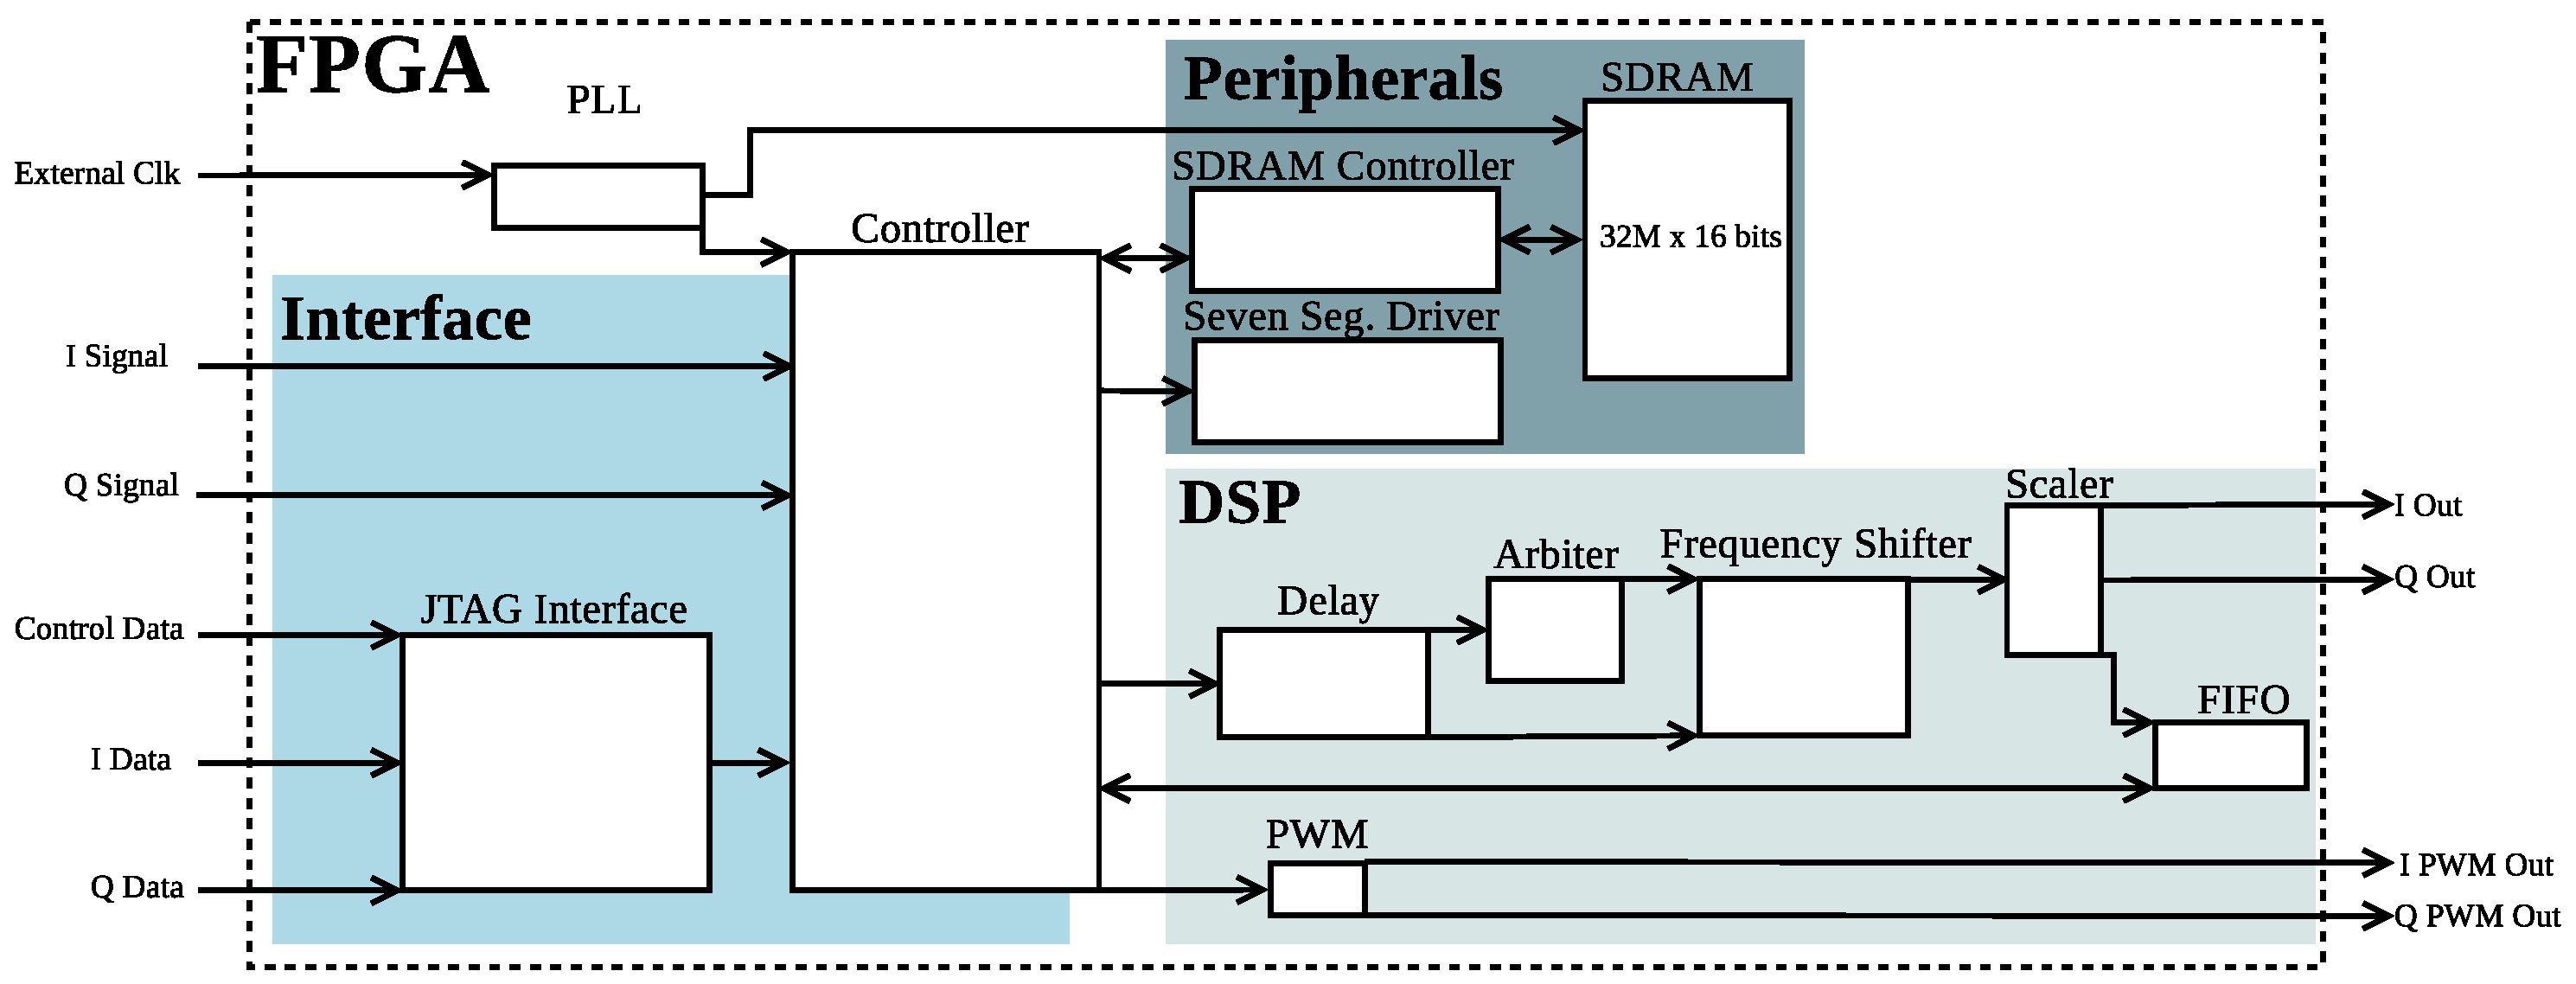
\includegraphics[width=0.95\linewidth]{img/System_Overview}
		\caption{Illustration of the implementation of the  FPGA based DRFM System}
		\label{fig:DRFM_Architecture}
	\end{figure*}
	
	\subsection{JTAG Interface}
		\noindent Joint Action Test Group (JTAG) was originally used as a simplified standard for interconnectivity testing for PCB manufacturing. It was created as a result of Integrated Circuits (IC) pins becoming more densely spaced and therefore classical interconnectivity test approaches were infeasible. The JTAG protocol mitigated the need for physical access to an IC's pins through the use of shift register chains.  \\ \newline In the JTAG standard (IEEE 1149.1) the collections of shift registers are referred to as Boundary Scan Cells (BSCs) which sample and hold data from and to the pin interface. As a result the BSCs can be configured into a serial shift chain thereby allowing to be driving by a serial interface. \\ \newline 	The JTAG interface implemented on the DRFM system allows for software based monitoring, updating and controlling of the DRFM system through the JTAG port.  Through the use of the Altera Virtual JTAG Intellectual Property (IP) core it is possible to access to the JTAG control signals that are routed to the FPGA core, which allow for a fine control over the JTAG resources thereby granting real-time general purpose serial communication \cite{JTAG}. \\ \newline	Through the use of  a Python {\color{red} maybe mention the pyqt model in a subsection} based User Interface (UI) that runs a TCL JTAG server it is possible to transfer both I/Q data as well as control information to the FPGA as may be seen in Fig.~\ref{fig:DRFM_Architecture}. The control word consists of 64 bits with flags and data contained within its length. The control word composition may be seen in Table.~\ref{tab:Control_Info} given that the most significant bit is at position 64.
		
		\begin{table}[h!]
			\centering
			\caption{Control Word Composition}
			\begin{tabular}{ccc}

				\textbf{Control Information} & \textbf{Control Flag Position} & \textbf{Control Data Length} \\ 
				Doppler Shift 	& 33 & 32  \\
				Time Delay    	& 44 & 10 \\
				Amplitude Scale & 61 & 16 
			\end{tabular}
		\label{tab:Control_Info}
		\end{table}
	
	\subsection{External Peripherals}
	\noindent In order to account for the requirement of I/Q data injection, an external SDRAM memory was incorporated into the DRFM system. It was used as a means to store the injected I/Q data in order to recall it for the DSP operations of the DRFM system. The SDRAM device is a 512Mb high speed CMOS dynamic access memory with 32M of address space that address 16 bit words \cite{SDRAM}. \\ \newline {\color{red} maybe discuss how I/Q data is dealt with in terms of inject. How only have 16bit words and each I/Q channel is 16 bits.} \\ \newline An SDRAM controller was implemented on the FPGA in order to facilitate communication with the external SDRAM peripheral. The controller made use of the Altera SDRAM Controller IP Core which uses the Avalon Interfacing standard to communicate with the SDRAM device. This was integrated into the system through the use of the Altera Qsys integration tool, that allowed for physical pin allocations to the external SDRAM device \cite{SDRAM_Core}. \\ \newline In addition to this it was required to clock the external SDRAM device at different clock rate. Therefore it was necessary to implement a Phase Locked Loop (PLL) in order to synchronously  step down the clock speed.\\ \newline Finally, for debugging and user interfacing purposes a group seven segment displays were used. The seven segment displays give visual feedback to the operator of the system by displaying the current state of the DRFM system.
	\subsection{Signal Processing}
	\noindent As previously discussed, the digital signal processing aspect of a DRFM system is critical to its operation. As time delays, frequency shifts and amplitude scalings are needed in order to emulate a target from a radar system's perspective. \\ \newline The major consideration in the implementation of this signal processing scheme was the order in which the signal processing operations were performed. This was due to the real-time processing requirements of a DRFM system, such when performing variable time delays there would be no loss of coherence between the input and output signals. This meant that if a time delay was set by the user and a frequency shift was then applied, the system should not have to repopulate the delay buffer. For this reason the order of the signal processing operations were to first perform the time-delay, then frequency shifts and finally amplitude scaling, as can be seen in Fig.~\ref{fig:DRFM_Architecture}. \\ \newline In order to describe the signal processing model the signal, $s(n)$, is considered to be the input to the signal processing chain. As the DRFM system receives I/Q data $s(n)$ may be  expressed mathematically as
	{\color{red}  THIS IS WRONG}
	\begin{equation}
		s(n) = v_{rx}(n)cos(2\pi f_{lo} n) + v_{rx}(n)sin(2\pi f_{lo} n) 
	\end{equation}
	\noindent where $v_{rx}(n)$ is the received RF signal and $f_{lo}$ is the local oscillator frequency.\\
		
	\subsubsection{Time Delay}
	 The time delay operation may be expressed as a method of altering the index of the input signal $s(t)$. This process may be summarized mathematically by
	\begin{equation}
		s_{delay}(k) = s(n -k),\quad n \geq k
	\end{equation}
	 \noindent This then may be implemented on a digital system by injecting a portion of the input signal $s(n)$ into a RAM. After which, it is possible to index previous values of $s(n)$ by means of the RAM's address pointers. Which then allows for the outputting of previous values of the inputted signal given that capacity criteria has been met. This being that the delay address index, $k$, is less than or equal to current RAM address index, $n$. In the implementation of the DRFM system, a dual port, 1024 address long, 16 bit wide RAM is implemented internally on the FPGA. \\ \newline The limitations of this are that 1024 samples must be maintained in the RAM, thereby inhibiting the DRFM system from being able to output data for first 1024 clock cycles of operation. Naturally, this is an overhead of any DRFM system as real-time data must be sampled and stored. However, once the capacity criteria of the RAM have been met a single sample may be outputted every clock cycle. \\ \newline For this reason, the signal processing chain was structured as it is. This was because had a user defined variable frequency shift occurred before the delay, the RAM would have had to be refilled as previous values of the frequency shifted signal would need to be outputted.  \\ \newline Finally, as the time delay control data word was specified to be 1024, it was necessary to maintain 1024 samples in the RAM at any point.\\
	\subsubsection{Frequency shifting}
	
		{ \color{red}  I OVER LOOKED THE FREQUENCY SHIFTED. NEED TO FIXED TOMORROW. }
		a \\ Principals of I/Q Data \\ Derive Mathematically how the shift works \\ 
	
	\subsubsection{Fractional Amplitude Scaling}
		a \\ input valies

	
	



